%! TEX root = ../main.tex
\documentclass[main]{subfiles}

\begin{document}
\chapter{はじめに}
自律移動が可能なAGV(Automatic Guided Vehicle)やAMR(Autonomous Mobile Robot)と呼称されるロボットの需要は高まってきており,
走行や工場内でのモノの運搬以外の用途で様々な環境への導入が進められている.
サービス業をはじめ,少子高齢化社会による人手不足解消を目的としたロボット導入は年々需要が増加しており,
より高度な作業やタスクをこなすことを目的としたロボットの開発や研究は多く行われている.

\section{研究背景}
    本章ではAGVやAMRについての現状や市場調査を行い, 内在する問題点について言及する. 
    \subsection{AGV, AMRの現状}
    \vspace{9pt}
    近年,自動運転技術の発展に伴い,様々な作業やタスクをこなす自律移動ロボットが導入されている.
    AGVとAMRの世界市場規模の推移を\Fig{fig:label1-1}に示す.
    2020年の新型コロナウイルス感染拡大による行動制限は,家に滞在する時間を増やし,世界各国のEC市場を拡大した.
    物流業界ではEC市場拡大に伴う物量増加や人手不足の対策として、物流自動化などを通じた倉庫内業務の効率化需要が高まり、
    AGV,AMRの導入拡大へと繋がったと考えられている.

    \begin{figure}[htbp]
        \centering
        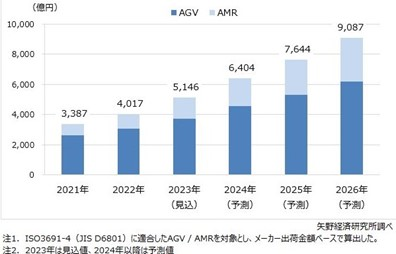
\includegraphics[keepaspectratio, width=0.6\linewidth]{figures/first/1_1_image.png}
        \caption{AGVとAMRの世界市場規模予測([1]より引用)}
        \label{fig:label1-1}
    \end{figure}

    \subsection{製造現場におけるAGV,AMRについて}
    \vspace{9pt}
    次にAGV,AMR導入が拡大されている物流倉庫,製造業の工場内の効率化に使用される機器について無線通信技術の側面に着目する.
    \Fig{fig:label1-2}(左)は製造現場における無線通信技術の使用例を示す.
    図2.2(右)は図2.2(左)に示された使用例の概要と想定される通信技術について示す.
    製造現場で稼働するロボットは遠隔での制御技術が用いられており,操縦者を必要とせず作業をこなす.
    図2.2(右)のそれぞれの使用例に想定される通信技術をみると主にWi-Fiとローカル5Gが大多数を占めている.

    今後,製造現場の効率がさらに求められると,通信の混線によるトラブルが懸念される.
    また,通信の混線を緩和するためにWi-Fiアクセス端末を増加させることは
    一時的な緩和につながるが, 将来的なコストの増加は避けられない.
    Wi-Fiを通信のベースとしたロボットではWi-Fiアクセス端末の通信範囲以上の稼働は見込めず,
    動的なWi-Fiアクセス端末の割り当て等が必要となり,スケーラビリティに欠けるという問題点も考えられる.

    \begin{figure}[htbp]
        \centering
        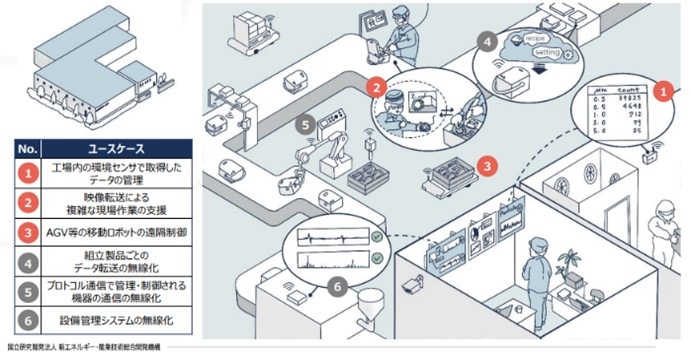
\includegraphics[keepaspectratio, width=0.6\linewidth]{figures/first/1_2_image_left.jpg}
        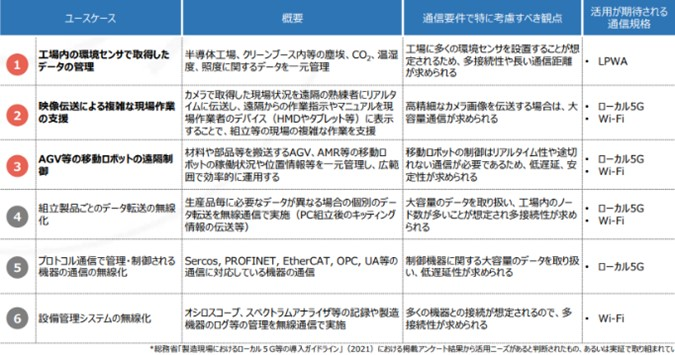
\includegraphics[keepaspectratio, width=0.6\linewidth]{figures/first/1_2_image_right.jpg}
        \caption{製造現場における無線通信技術の使用例(図上),その概要や想定される通信技術(図下) ([2]より引用)}
        \label{fig:label1-2}
    \end{figure}

\end{document}